\documentclass{beamer}
\usepackage[utf8]{inputenc}
\usepackage[T1]{fontenc}
\usepackage[french]{babel}
\usepackage{amsmath}
\usepackage{amssymb}
\usepackage{tikz}
\usepackage{animate}
\usepackage{graphicx}
\usepackage{caption}
\usetheme{Madrid}
\usecolortheme{default}

\title{Modélisation du transfert thermique et de masse dans la pyrolyse du bois}
\author{Julien Léger, Simon Francheo, Gurwan Le Hebel, Pierre Mériaux}
\institute{ENSEIRB-Matmeca, Filière Mathématiques et Mécanique 1ère année}
\date{13 Mai 2025} 


\usetheme{Madrid}
\usecolortheme{default}

\begin{document}



\begin{frame}[plain]
    \titlepage

    \vfill
    \centering
        \parbox{0.4\textwidth}{
            \centering \footnotesize \textbf{Encadrants :}\\
            Ludovic Godard-Cadillac\\
            Thanh-Ha Nguyen-Bui
        }
\end{frame}

\author{J. Léger, S. Francheo, G. Le Hebel, P. Mériaux}
\begin{frame}{Introduction}
    \begin{itemize}
        \item Enjeu : Sécurité incendie en forêt et pour les constructions.
        \item Modèle : Couplage des réactions chimiques de pyrolyse et de la diffusion de la chaleur.
        \item Utilisation de schémas implicites (Euler implicite, Crank-Nicolson)
    \end{itemize}
\end{frame}

\begin{frame}{Équations de conservation de la masse}
    \begin{equation}
        \left\lbrace
            \begin{aligned}
                \frac{\partial \rho_b}{\partial t} &= -(k_1 + k_2)\rho_b \\
                \frac{\partial \rho_c}{\partial t} &= k_1\rho_b\\
                \frac{\partial \rho_g}{\partial t} &= k_2\rho_b\\
                \frac{\partial \rho_l}{\partial t} &= -k_3\rho_l\\
                \frac{\partial \rho_v}{\partial t} &= k_3\rho_l\\
            \end{aligned}
        \right.
    \end{equation}
    \begin{itemize}
        \item $\rho_b, \rho_c, \rho_g, \rho_l, \rho_v$ : masses volumiques du bois, du charbon, du gaz, du liquide et de la vapeur.
        \item $k_1, k_2, k_3$ : taux de réactions chimiques.
    \end{itemize}
\end{frame}

\begin{frame}{Résolution numérique}
    \begin{itemize}
        \item Schémas numériques : Euler implicite et Crank-Nicolson.
        \item Condition de Dirichlet ($T(t) = 300 + a \cdot t$).
    \end{itemize}
    \begin{figure}
        \centering
        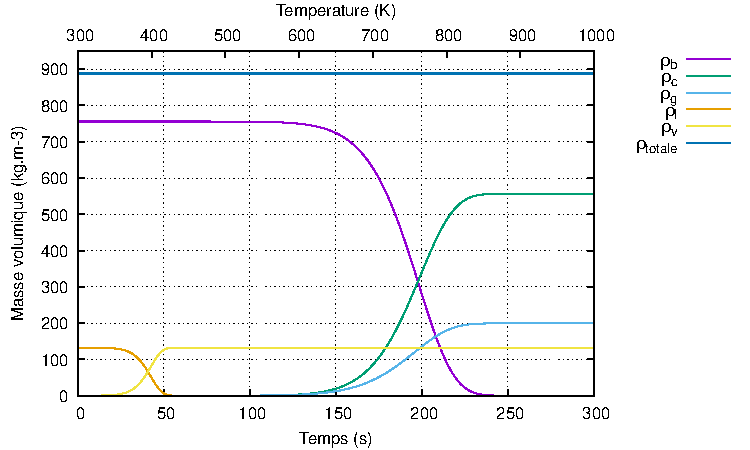
\includegraphics[width=0.8\linewidth]{images/densite_CK2.pdf}
        \caption{Évolution des masses volumiques avec le schéma de Crank-Nicolson}
    \end{figure}
\end{frame}

\begin{frame}{Étude de l'erreur}
    \begin{itemize}
        \item Comparaison des erreurs numériques locales entre Euler implicite et Crank-Nicolson.
        \item Le schéma de Crank-Nicolson est plus précis que celui d'Euler implicite.
    \end{itemize}
    \begin{minipage}{0.48\linewidth}
        \centering
        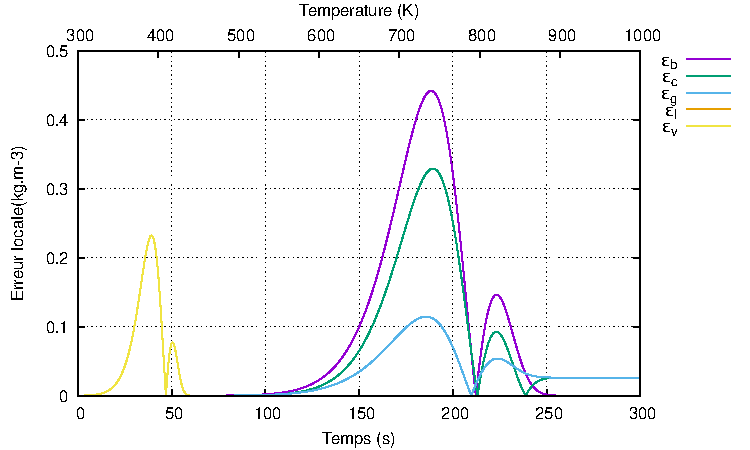
\includegraphics[width=\linewidth]{images/error_EI.pdf}
        
        \vspace{0.5em}
        {\small Erreur locale – Euler implicite}
    \end{minipage}
    \hfill
    \begin{minipage}{0.48\linewidth}
        \centering
        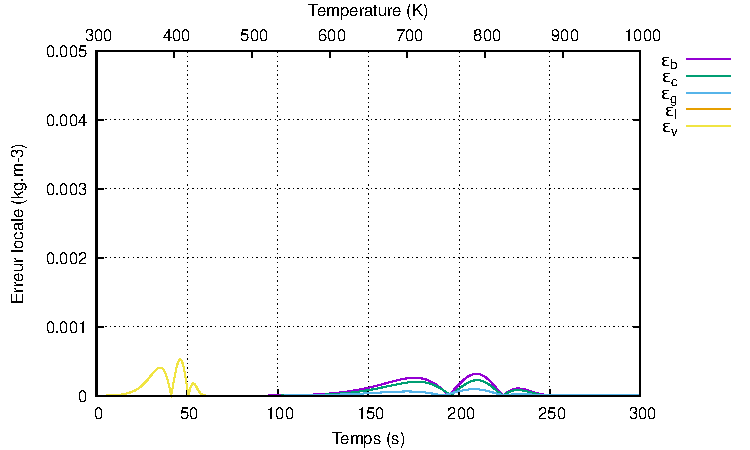
\includegraphics[width=\linewidth]{images/error_CK2.pdf}
        
        \vspace{0.5em}
        {\small Erreur locale – Crank-Nicolson}
    \end{minipage}
\end{frame}

\begin{frame}{Équation de la chaleur}
    \begin{equation}
        \frac{\partial T}{\partial t} =    \frac{\lambda}{ \rho C_p} \frac{\partial^2 T}{\partial x^2} + Q_r
    \end{equation}
    \begin{itemize}
        \item $\lambda$, $\rho$, $C_p$ : conductivité thermique, densité, chaleur spécifique.
        \item $Q_r$ : terme source de chaleur.
        \item EDP linéaire par rapport à T
        \item Schéma numérique retenu (avec $\lambda=\rho=D=1$ et $Q_r=0$) : 
        \begin{equation}
            \frac{T_i^{n+1}-T_i^n}{\Delta t}= \frac{T_{i+1}^n+T_{i-1}^n-2T_i^{n+1}}{\Delta x^2} 
        \end{equation}
    \end{itemize}
\end{frame}

\begin{frame}{Résultats et interprétations}
    \begin{itemize}
        \item Évolution du champ de température.
        \item Validation du modèle par comparaison avec des solutions analytiques.
        \item Condition de Dirichlet : $ T(t, x=0) = 280K$ et $T(t, x=L) = 280K$
    \end{itemize}
    \begin{figure}
        \centering
        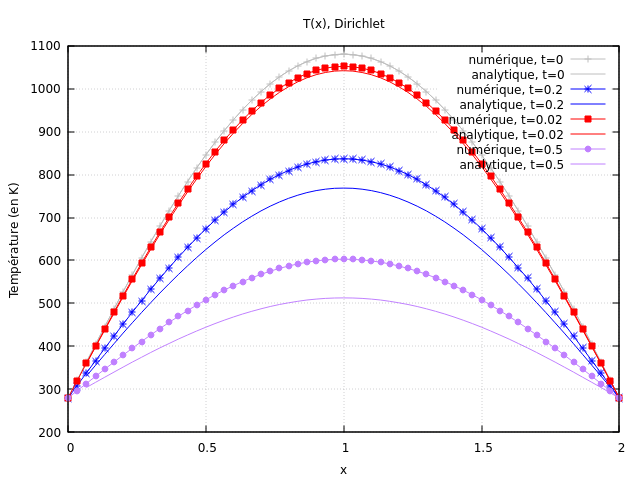
\includegraphics[width=0.75\linewidth]{images/graphe_temperature_grid.png}
        \caption{Température le long d'un segment étudié en des temps différents}
    \end{figure}
\end{frame}

\begin{frame}{Deuxième condition}
    \begin{itemize}
        \item Condition de Dirichlet à gauche $ T(t, x=0) = 800K$
        \item Condition de Neumann à droite $
            \frac{\partial T}{\partial x}]_{x=L} = 0$
        
    \end{itemize}
    \begin{figure}
        \centering
        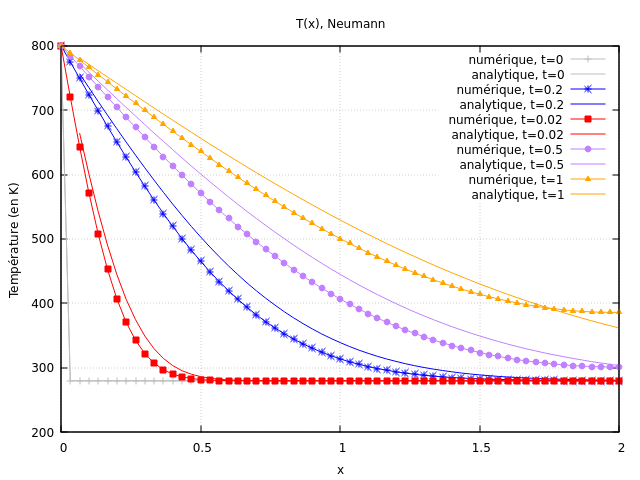
\includegraphics[width=0.75\linewidth]{images/graphe_temperature_Neumann_1.png}
        \caption{Graphe avec condition de Neumann}
    \end{figure}
\end{frame}

\begin{frame}{Couplage}
    \begin{itemize}
        \item Équation de la chaleur sous forme complète :
        \begin{equation}
            \rho C_p \frac{\partial T}{\partial t} = \nabla(\lambda \nabla T) + Q_r
        \end{equation}
        \item Coefficients $\rho$, $\lambda$ dépendant de T $\Longrightarrow$ EDP non linéaire
    \end{itemize}
    
    \begin{itemize}
        \item \textbf{1D :} Maillage régulier en espace de $Nx + 2$ points.
        \item Approximation du flux thermique ($\lambda \nabla T$) aux milieux des mailles.
        \item Méthodes implicites pour garantir la stabilité du schéma et améliorer le temps de calcul.
    \end{itemize}
    \begin{block}{Conditions initiales et aux limites}
        \begin{itemize}
            \item Condition initiale : $T(0,x) = T_{\text{init}}(x) = 300 K$
            \item Condition de Dirichlet à gauche : $T(t, x=0) = T_G = 800 K$
            \item Condition de Neumann adiabatique à droite : $\left. \frac{\partial T}{\partial x} \right|_{x = L} = 0$
        \end{itemize}
    \end{block}
    
\end{frame}


\begin{frame}{Schéma d'Euler implicite à 3 points}
    \begin{equation}
        - \beta_{i-1}^{n} T_{i-1}^{n+1} + (1 + \alpha_i^n) T_i^{n+1} - \beta_{i+1}^{n} T_{i+1}^{n+1} = T_i^n + \gamma_i^n Q_i^n
    \end{equation}
    \begin{itemize}
        \item \footnotesize $\beta_{i \pm 1}^{n} = \frac{\Delta t}{\Delta x^2} \frac{\lambda_{i \pm \frac{1}{2}}^n}{(\rho C_p)_i^n}$, \quad $\alpha_i^n = \frac{\Delta t}{\Delta x^2 (\rho C_p)_i^n} \left( \lambda_{i - \frac{1}{2}}^n + \lambda_{i + \frac{1}{2}}^n \right)$, \quad $\gamma_i^n = \frac{\Delta t}{(\rho C_p)_i^n}$

        \begin{itemize}
        \item Discrétisation sous forme matricielle MOL.
        \item Résolution d'un système d'équations différentielles ordinaires :
        \end{itemize}
        \begin{equation}
            (I + A) \cdot T^{n+1} = b
        \end{equation}

        \begin{block}{Matrice A et second membre b}
            \footnotesize{ 
            \[
            A =
            \begin{bmatrix}
            \alpha_1^n & -\beta_2^n & 0 & \cdots & 0 \\
            -\beta_1^n & \alpha_2^n & -\beta_3^n & \cdots & 0 \\
            0 & \ddots & \ddots & \ddots & 0 \\
            \vdots & \cdots & -\beta_{Nx-2}^n & \alpha_{Nx-1}^n & -\beta_{Nx}^n \\
            0 & \cdots & 0 & -\beta_{Nx-1}^n & \beta_{Nx}^n
            \end{bmatrix}, \qquad
            b =
            \begin{bmatrix}
            T_1^n + \beta_{0}^n T_G + \gamma_1^n Q_1^n \\
            T_2^n + \gamma_2^n Q_2^n  \\
            \vdots \\
            \vdots \\
            T_{Nx}^n + \gamma_{Nx}^n Q_{Nx}^n
            \end{bmatrix}
            \]}
        \end{block}
    \end{itemize}
\end{frame}

\begin{frame}{Schéma de Crank-Nicolson à 3 points}
    \footnotesize{
    \begin{equation}
        - \frac{\beta_{i-1}^{n}}{2} T_{i-1}^{n+1} + \left(1 + \frac{\alpha_i^n}{2} \right) T_i^{n+1} - \frac{\beta_{i+1}^n}{2} T_{i+1}^{n+1} = \frac{\beta_{i-1}^n}{2} T_{i-1}^{n} + \left(1 - \frac{\alpha_i^n}{2} \right) T_i^{n} + \frac{\beta_{i+1}^n}{2} T_{i+1}^{n} + \gamma_i^n Q_i^n
    \end{equation}}


    \begin{itemize}
        \item Schéma d'ordre 2 global.
        \item Résolution sous forme matricielle.
    \end{itemize}

    \begin{equation}
            (I + \frac{1}{2}A) \cdot T^{n+1} = (I - \frac{1}{2}A)T^n + \gamma^n \cdot Q^n
    \end{equation}

    \begin{block}{}
        \begin{itemize}
        \item \textbf{Solveur linéaire :} Méthode LU adapté aux matrices tridiagonales
        \item Complexité en O(n)
        \end{itemize}
    \end{block}
\end{frame}

\begin{frame}{Principe de l'algorithme}
    \begin{block}{Pseudo-code résumé}
        \begin{enumerate}
            \item Initialisation :
            \begin{itemize}
                \item Initialisation des constantes de réaction
                \item Initialisation des masses volumiques
                \item Calcul de $\Delta x$ et $\Delta t$.
                \item Initialisation des températures.
            \end{itemize}
            \item Schéma numérique :
            \begin{itemize}
                \item Calcul de $\rho C_p$, $\lambda$, et $Q_r$.
                \item Selon le schéma choisi (Euler implicite, Crank-Nicolson) :
                \begin{itemize}
                    \item Remplissage de la matrice $A$ et construction du second membre $b$.
                    \item Résolution du système $A \cdot T^{n+1} = b$.
                    \item Application des conditions aux limites.
                \end{itemize}
                \item Mise à jour des masses volumiques.
                \item Enregistrement des données au temps $t_n$.
            \end{itemize}
            \item Mise à jour des températures et incrémentation du temps.
        \end{enumerate}
    \end{block}
\end{frame}

\begin{frame}{Résultats du couplage en 1D}
    \begin{figure}
        \centering
        \animategraphics[autoplay,loop,controls,width=0.8\textwidth]{5}{images/1D/temp_}{01}{41}
        \caption{\centering \footnotesize Évolution de la température et des masses volumiques en 1D avec Crank-Nicolson}
    \end{figure}
    \begin{itemize}
        \item Corrélation cohérente entre la température et les masses volumiques.
        \item Formation de charbon et de gaz à gauche du domaine.
    \end{itemize}
\end{frame}

\begin{frame}{Cas bidimensionnel}
    \begin{itemize}
        \item Construction d'un schéma d'EI pour l'équation de la chaleur en 2D.
        \begin{equation}\label{CouplageEI2D} \footnotesize{ 
            (1 + \alpha_{i,j}^n) T_{i,j}^{n+1} = T_{i,j}^{n} + \beta_{i+1}^{n} T_{i+1,j}^{n+1} + \beta_{i-1}^{n} T_{i-1,j}^{n+1} + \beta_{j+1}^{n} T_{i,j+1}^{n+1} + \beta_{j-1}^{n} T_{i,j-1}^{n+1} + \gamma_{i,j}^n Q_{i,j}^n}
        \end{equation}
        \item Méthode itérative de Gauss-Seidel pour la résolution.
        \end{itemize}
        \begin{center}
        \begin{tikzpicture}[scale=0.5]
        
        \def\nx{12}
        \def\ny{9}
        \def\dirStart{3}
        \def\dirEnd{6.75}
        
        \draw[step=0.8cm,gray!30,very thin] (0,0) grid ({(\nx+1)*0.8},{(\ny+1)*0.8});
        
        \draw[very thick] (0,0) rectangle ({(\nx+1)*0.8},{(\ny+1)*0.8});
        
        \draw[line width=3pt,red] (0,{0.7*\dirStart}) -- (0,{0.9*\dirEnd});
        \node[red,rotate=90,anchor=south] at (-0.4,{0.8*(\dirStart+\dirEnd)/2}) {$\boxed{T = 1000\,\text{K}}$};
        
        \draw[line width=2pt,blue] (0,0) -- (0,{0.7*\dirStart});
        \draw[line width=2pt,blue] (0,{0.9*\dirEnd}) -- (0,{0.8*(\ny+1)});
        \draw[line width=2pt,blue] ({0.8*(\nx+1)},0) -- ({0.8*(\nx+1)},{0.8*(\ny+1)});
        \draw[line width=2pt,blue] (0,0) -- ({0.8*(\nx+1)},0);
        \draw[line width=2pt,blue] (0,{0.8*(\ny+1)}) -- ({0.8*(\nx+1)},{0.8*(\ny+1)});
        
        \node[blue,rotate=90] at ({0.8*(\nx+1)+0.7},{0.8*(\ny+1)/2}) {\large $\frac{\partial T}{\partial x} = 0$};
        \node[blue] at ({0.8*(\nx+1)/2},-0.7) {\large $\frac{\partial T}{\partial y} = 0$};
        \node[blue] at ({0.8*(\nx+1)/2},{0.8*(\ny+1)+0.7}) {\large $\frac{\partial T}{\partial y} = 0$};
        
        \node at ({0.8*(\nx+1)/2},{0.8*(\ny+1)/2}) {\textbf{CI} :  $T_0 = 300\,\text{K}$};
        
        \draw[->,thick] (-0.2,0) -- ({0.8*(\nx+1)+0.5},0) node[right] {$x$};
        \draw[->,thick] (0,-0.2) -- (0,{0.8*(\ny+1)+0.5}) node[above] {$y$};
        
        \node at ({0.8*(\nx+1)},-0.5) {$nx+1$};
        \node at (-1.4,{0.8*(\ny+1)}) {$ny+1$};
        
        \end{tikzpicture}
        \end{center}
    
    
\end{frame}

\begin{frame}{Cas bidimensionnel : 1er Exemple}

    \begin{figure}
        \centering
        \makebox[\textwidth][c]{
        \animategraphics[autoplay,loop,controls,width=1.05\textwidth]{5}{images/2D/multiplot_}{01}{41}
        }
        \caption{\centering \footnotesize Évolution des champs de température et de masse volumique du charbon en 2D}
    \end{figure}
\end{frame}

\begin{frame}{Cas bidimensionnel : 2ème Exemple}

    \begin{center}
    \begin{tikzpicture}[scale=0.7]
    
    \def\nx{12}
    \def\ny{9}
    \def\dirStart{0}
    \def\dirEnd{\ny+1}
    
    \draw[step=0.8cm,gray!30,very thin] (0,0) grid ({(\nx+1)*0.8},{(\ny+1)*0.8});
    
    \draw[very thick] (0,0) rectangle ({(\nx+1)*0.8},{(\ny+1)*0.8});
    
    \draw[line width=3pt,red] (0,{0.8*\dirStart}) -- (0,{0.8*\dirEnd});
    \node[red,rotate=90,anchor=south] at (-0.4,{0.8*(\dirStart+\dirEnd)/2}) {\large $\boxed{T = 800\,\text{K}}$};
    
    \draw[line width=2pt,blue] ({0.8*(\nx+1)},0) -- ({0.8*(\nx+1)},{0.8*(\ny+1)});
    \draw[line width=2pt,blue] (0,0) -- ({0.8*(\nx+1)},0);
    \draw[line width=2pt,blue] (0,{0.8*(\ny+1)}) -- ({0.8*(\nx+1)},{0.8*(\ny+1)});
    
    \node[blue,rotate=90] at ({0.8*(\nx+1)+0.5},{0.8*(\ny+1)/2}) {\large $\frac{\partial T}{\partial x} = 0$};
    \node[blue] at ({0.8*(\nx+1)/2},-0.5) {\large $\frac{\partial T}{\partial y} = 0$};
    \node[blue] at ({0.8*(\nx+1)/2},{0.8*(\ny+1)+0.5}) {\large $\frac{\partial T}{\partial y} = 0$};
    
    \draw[dashed,thick] (0,{0.8*(\ny+1)/2}) -- ({0.8*(\nx+1)},{0.8*(\ny+1)/2});
    
    \node at ({0.8*(\nx+1)/2},{0.8*(\ny+1)*3/4}) {\textbf{Bois de pin, $T_0 = 300\,\text{K}$}};
    \node at ({0.8*(\nx+1)/2},{0.7*(\ny+1)*3/4}) {\textbf{$\rho_{b,0} = 360\,\text{kg/m$^3$} $}};
    \node at ({0.8*(\nx+1)/2},{0.8*(\ny+1)*1/4}) {\textbf{Bois de chêne, $T_0 = 300\,\text{K}$}};
    \node at ({0.8*(\nx+1)/2},{0.5*(\ny+1)*1/4}) {\textbf{$\rho_{b,0} = 888\,\text{kg/m$^3$} $}};
    \draw[->,thick] (-0.2,0) -- ({0.8*(\nx+1)+0.5},0) node[right] {$x$};
    \draw[->,thick] (0,-0.2) -- (0,{0.8*(\ny+1)+0.5}) node[above] {$y$};
    s
    \node at ({0.8*(\nx+1)},-0.5) {$nx+1$};
    \node at (-1,{0.8*(\ny+1)}) {$ny+1$};
    
    \end{tikzpicture}
    \end{center}
\end{frame}

\begin{frame}{Cas bidimensionnel : 2ème Exemple}

    \begin{figure}
        \centering
        \animategraphics[autoplay,loop,controls,width=0.6\textwidth]{5}{images/2D_2W/temp_}{01}{41}
        \caption{\footnotesize Évolution des champs de température en 2D avec 2 bois}
    \end{figure}
\end{frame}

\begin{frame}{Temps de calcul}
    \begin{block}{Comparaison des temps d'exécution}
        \begin{itemize}
            \item \textbf{1D, Euler Implicite} : 0.25 secondes
            \item \textbf{1D, Crank-Nicolson} : 0.33 secondes
            \item \textbf{2D, Euler Implicite} : 305.60 secondes
            \item \textbf{2D avec deux bois, Euler Implicite} : 299.80 secondes
        \end{itemize}
    \end{block}
    \begin{itemize}
        \item Différence négligeable entre les schémas 1D
        \item Passage à la 2D multiplie exponentiellement les temps de calcul
    \end{itemize}
    \begin{block}{}
        \textbf{$\Longrightarrow$ Parallélisation pour des problèmes plus grands}
    \end{block}
\end{frame}

\begin{frame}{Conclusion}
    \begin{itemize}
        \item Modélisation et simulation numérique de la pyrolyse du bois.
        \item Utilisation de schémas implicites pour étudier l'évolution des champs de température et des masses volumiques.
        \item Résultats cohérents avec les attentes physiques.
    \end{itemize}
\end{frame}

\end{document}
